% Random Forest varies greatly
Before beginning analysis on the classifiers in general, it is important to mention that this year was a statistical anomaly as far as the NCAA Tournament is concerned.  
To illustrate this, since 1985 (the year the tournament became what it is today), there have only been four years that a 12 seed team has not beaten a 5 seed team: 1988, 2000, 2007, and this year, 2018.  
Second, since 1985, there have only been four teams that were ranked as an 11 seed that made it to the final four: LSU in 1986, George Mason in 2006, VCU in 2011, and Loyola-Chicago in 2018.  
Finally, and also since 1985, there has only been one instance of a 16 seed team beating a 1 seed team: this year, UMCB upset Virginia.  
Not only was Virginia the national favorite to win the tournament (most people in the U.S. picked them to win the championship) but they were also highly ranked by every other ranking algorithm researched.  
All three of these individually anomalous things happened this year.  
This helps illustrate the difficulty of trying to correctly predict the NCAA tournament.  
There will always be an element of randomness that cannot be predicted, regardless of the techniques used.  

Of the "out of the box" classifiers used, the ones that performed the best the most consistently are the LR classifier and the SVM classifier.  
When tested on the 2017 data, they achieved an accuracy of about $72.6\%$, which is about what other models have achieved.  
In the 2018 tournament, they finished with $850$ and $860$ points respectively, which would place them above the $80^{th}$ percentile in the nation.  
While the RF classifier can outperform them, it's success is varied and random, and thus much less reliable.  
This was easy enough to determine from the 2017 data testing, as on different runs, the parameters that gave the best results changed on practically every single iteration.  
Thus, the choice of picking the best parameters alone is a guess that can greatly effect the success of the RF model.  
In fact, it sometimes does just as poorly as the GNB classifier, which, of the regular classifiers, is by far the worst.  
This was actually a little surprising, since it tested almost as well as the LR classifier on the 2017 data, coming in at approximately $72.2\%$.  
This may be due to the fact that this year was rather anomalous, or it could just be that in 2017 it performed extraordinarily well.  
Unsurprisingly, the MYC classifier was by far the worst.  
While it did perform better than random, it still has a lot of adjusting that needs to happen before it can adequately compete with any of the other classifiers.  
Reversing the predictions of the MYC classifier also doesn't significantly improve the score.  
This is because it's just a little better than random, and as such, wouldn't have any better chances in later rounds by switching it's previous decisions.  
To illustrate this point, the expected value for a randomly guessed bracket is the sum of the number of games predicted, times the probability of guessing that game correctly, times the score for that game.  
However, it's important that we exclude any round where it's expected score is smaller than the points that would be awarded for correctly guessing a single game.  
Since this happens from the elite eight onward, the expected value is computed by
\begin{align*}
\mathbb{E}[x] &= \sum_{i=1}^{3} 2^{6-i}\left(\frac{1}{2^{i}}\right)\left(2^{i-1}\right)*10 \\
&= \sum_{i=1}^{3} 2^{5-i}*10 \\
&= 280
\end{align*}
The MYC classifier got $360$ points, which is $80$ points higher.  
The others are much better, and while they don't perform as close to perfect as desired, still manage to get into the higher percentiles.  
The other metric used to evaluate the classifier's success was the number of games guessed correctly (GGC), as well as the number of games that the classifier couldn't get right, because of previous guesses.  
That is, how times did the classifier pick a team that had already been eliminated in previous rounds.  
These games are referred to as "Impossible Games" (or IGs) because they were impossible for the classifier to correctly predict.  
Likewise, the points from those games are referred to as "Impossible Points" (or IPs).  
\begin{figure}[h!]
\centering
\caption{Games Guessed Correctly vs Impossible Games}
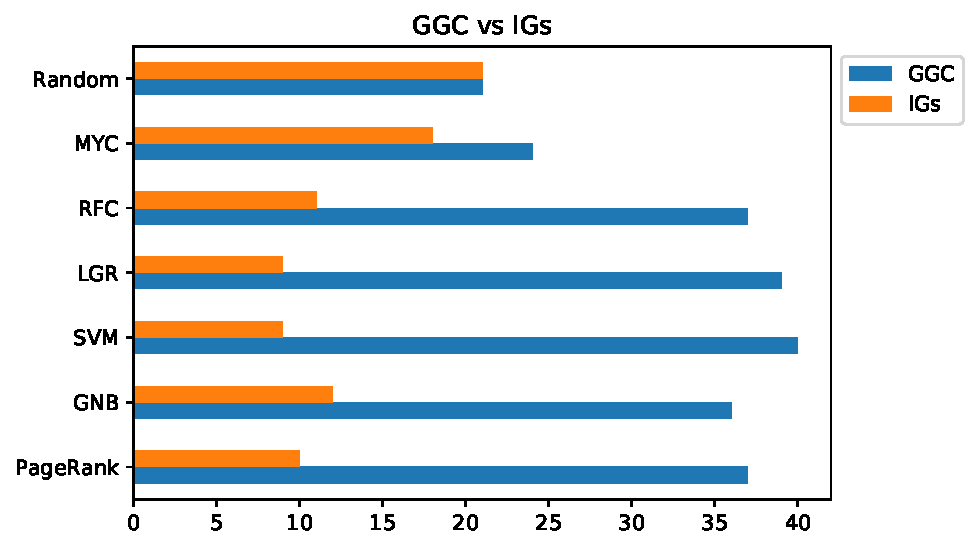
\includegraphics[height=0.35\textwidth,width=0.5\textwidth]{../GGC_vs_IGs.pdf}
\label{fig:istats1}
\end{figure}
\begin{figure}[h!]
\centering
\caption{Impossible Points for Each Classifier}
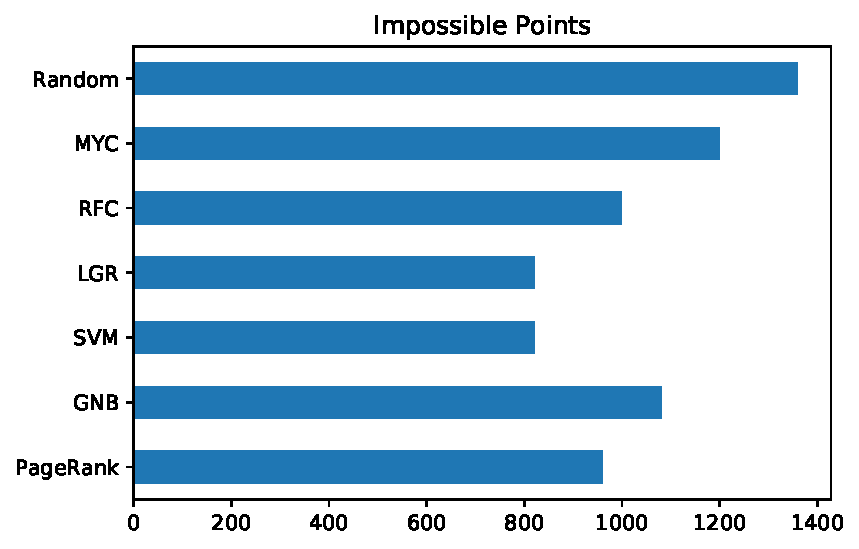
\includegraphics[height=0.35\textwidth,width=0.5\textwidth]{../Impossible_Points.pdf}
\label{fig:istats2}
\end{figure}
Those a comparison of those values are displayed in Figure \ref{fig:istats1} and Figure \ref{fig:istats2}.\newline\newline
%\begin{tabular}{|c|c|c|c|}
%\hline
%Classifier & \# of GGC & \# of IGs & IPs \\
%\hline
%PgRnk & 37 & 10 & 960 \\
%GNB & 36 & 12 & 1080 \\
%SVM & 40 & 9 & 820 \\
%LR & 39 & 9 & 820 \\
%RF & 36 & 10 & 980 \\
%MYC & 24 & 18 & 1200 \\
%Rand & 21 & 21 & 1360 \\
%\hline
%\end{tabular}  \newline\newline
The random values were calculated using the fact that $\left(1-\frac{1}{2^{i-1}}\right)\%$ of games for each of round $i=2,...,6$ should be impossible games.  
Again, it's important to note that the RF classifier varies, and can performs better than the LR classifier at times, as well as worse than the GNB classifier.  
In this metric, the LR model again consistently performs the best (with few exceptions from arbitrary runs of the RF classifier), followed by the PageRank classifier with the GNB classifier next, closely followed by the SVM classifier.  
So for this tournament, the GNB classifier correctly predicted more of the early games, but then the SVM  classifier correctly guessed more of the heavier weighted games later on, resulting in a higher overall score (which is evidenced from Figure \ref{fig:scores1}).  
All of them, though, are better than the expected value of randomly guessing.  